\documentclass[12pt,a4paper]{extreport}
\usepackage[utf8]{inputenc}
\usepackage[french]{babel}
\usepackage[T1]{fontenc}
\usepackage{amsmath}
\usepackage{amsfonts}
\usepackage{amssymb}
\usepackage{graphicx}
\author{Sébastien Hervieu}
\title{Contrôle Continu Problèmes Inverses: Régression Linéaire}
\renewcommand{\thesection}{\alph{section}}
\begin{document}
\maketitle

\section{Equation Linéaire}

Nous disposons de données $d(t,y)$ contenant les hauteurs $y$ du projectile à des instants $t$.
Par ailleurs, le modèle que nous voulons trouver est de la forme:
\[y(t)=m_1+m_2t-\frac{1}{2}m_3t^2\]

Nous posons donc l'équation suivante:
\begin{gather}
d = Gm
\end{gather}

et donc 

\begin{gather}
	\begin{bmatrix} y_1 \\ y_2 \\ \vdots \\ y_{25} \end{bmatrix}
	=
	\begin{bmatrix}
	1 & t_1 & -\frac{1}{2}t_1^2 \\
	1 & t_2 & -\frac{1}{2}t_2^2 \\ 
	\multicolumn{3}{c}{$\vdots$} \\
	1 & t_{25} & -\frac{1}{2}t_{25}^2
	\end{bmatrix}
	\begin{bmatrix} m_1 \\ m_2 \\ m_3 \end{bmatrix}
\end{gather}
où les $y_i$ et les $t_i$, $(i= 1, \dots, 25)$  sont les données et les $m_n$, $(n =1, 2, 3)$ sont les inconnues.


\section{Solution des moindres carrés, matrices de covariance et de corrélation}

La solution des moindres carrés est donnée par :
\begin{equation}
	\begin{gathered}
		m = (G^TG)^{-1}G^Td
	\end{gathered}\label{eq:1}
\end{equation}

En résolvant numériquement à l'aide de scilab, nous obtenons:
\begin{equation}
\begin{array}{c}
m_1 = 21396.743 \\[\jot] m_2 = 16.811659 \\[\jot] m_3 = 3.7141271
\end{array}
\end{equation}

\subsection*{Matrice de covariance des données}
En utilisant la formule donnée en \eqref{eq:1} pour le calcul des paramètres, nous faisons l'hypothèse implicite que l'erreur sur les données $\sigma$ est telle que 
\begin{gather}
\sigma^2 = 1
\end{gather}
Dans cette hypothèse la matrice de covariance des données $C_d$ est égale à la matrice identité $I$, soit:

\begin{gather}
	C_d =
	\begin{bmatrix}
	\sigma_1^2 & 0 & \dots & 0 \\
	0 & \sigma_2^2 & \dots & 0 \\
	\multicolumn{3}{c}{$\vdots$} \\
	0 & 0 & \dots & \sigma_{25}^2
	\end{bmatrix}
	=
	\begin{bmatrix}
	1 & 0 & \dots & 0 \\
	0 & 1 & \dots & 0 \\
	\multicolumn{3}{c}{$\vdots$} \\
	0 & 0 & \dots & 1 
	\end{bmatrix}
	= I
\end{gather}

\subsection*{Matrices de covariance du modèle}
La matrice de covariance du modèle $C_m$ est donnée de manière générale par:
\begin{gather}
	C_m = (G^TC_d^{-1}G)^{-1}
\end{gather}

Dans notre hypothèse où $C_d = I$, $C_m$ devient:
\begin{gather}
	C_m = (G^TG)^{-1}
\end{gather}

$C_m$ est calculée à l'aide de scilab; nous obtenons le résultat suivant:

\begin{gather}
	C_m =
	\begin{bmatrix}
		0.3654177 & -0.0120938 & -0.0001784 \\
  		-0.0120938 &  0.0005567 &  0.0000097 \\
  		-0.0001784 &  0.0000097  & 0.0000002
	\end{bmatrix}
\end{gather}

La matrice de corrélation des paramètres est donnée par la formule suivante:
\begin{gather}
	\rho_{ij} = \frac{C_m(m_i,m_j)}{\sigma_i\sigma_j}
\end{gather}
ce qui nous donne dans notre cas:
\begin{gather}
	CorrM =
	\begin{bmatrix}
	1 &-0.8479488 & -0.6838399 \\
  -0.8479488  & 1.        &  0.9535659 \\
  -0.6838399 &  0.9535659  & 1.  
	\end{bmatrix}
\end{gather}

\subsection*{Interpretation}
Nous constatons que $Cm$ n'est pas diagonale, qu'aucune valeur de la matrice de $CorrM$ n'est nulle.

\section{Estimation des paramètres avec $\chi_{\nu=1,p=0.95}^2$}
En effectuant le calcul suivant:
\begin{gather}
	\Delta m = \sqrt{\chi_{\nu=1,p=0.95}^2 \times diag(C_m)}
\end{gather}

avec $\chi_{\nu=1,p=0.95}^2 = 3.96$


nous obtenons les estimations des paramètres suivantes, avec leurs intervalles de confiance à 95\% projetés en 1D:

\begin{equation}
	\begin{array}{c}
		m_1 = 21396.743 \pm 1.2029356\;m\\
		[\jot] m_2 = 16.811659 \pm 0.046951\;m/s\\
		[\jot] m_3 = 3.7141271 \pm 0.0008587\;m/s^2
	\end{array}
\end{equation}

\section{Estimation des paramètres avec $\chi_{\nu=2,p=0.95}^2$}
En effectuant un calcul similaire au précédent:

\begin{gather}
	\Delta m = \sqrt{\chi_{\nu=2,p=0.95}^2 \times diag(C_m)}
\end{gather}

avec $\chi_{\nu=2,p=0.95}^2 = 5.99$


nous obtenons les estimations des paramètres suivantes, avec leurs intervalles de confiance à 95\% 3D projetés en 2D:

\begin{equation}
	\begin{array}{c}
		m_1 = 21396.743 \pm 1.4794769\;m\\
		[\jot] m_2 = 16.811659 \pm 0.0577445\;m/s\\
		[\jot] m_3 = 3.7141271 \pm 0.0010561\;m/s^2
	\end{array}
\end{equation}

\section{Tracé des ellipses de confiance à 0.95 pour les 3 combinaisons de paramètres}

Les ellipses de confiance à 0.95 pour les 3 combinaisons de paramètres sont les suivantes:

\begin{figure}[h]
\begin{center}
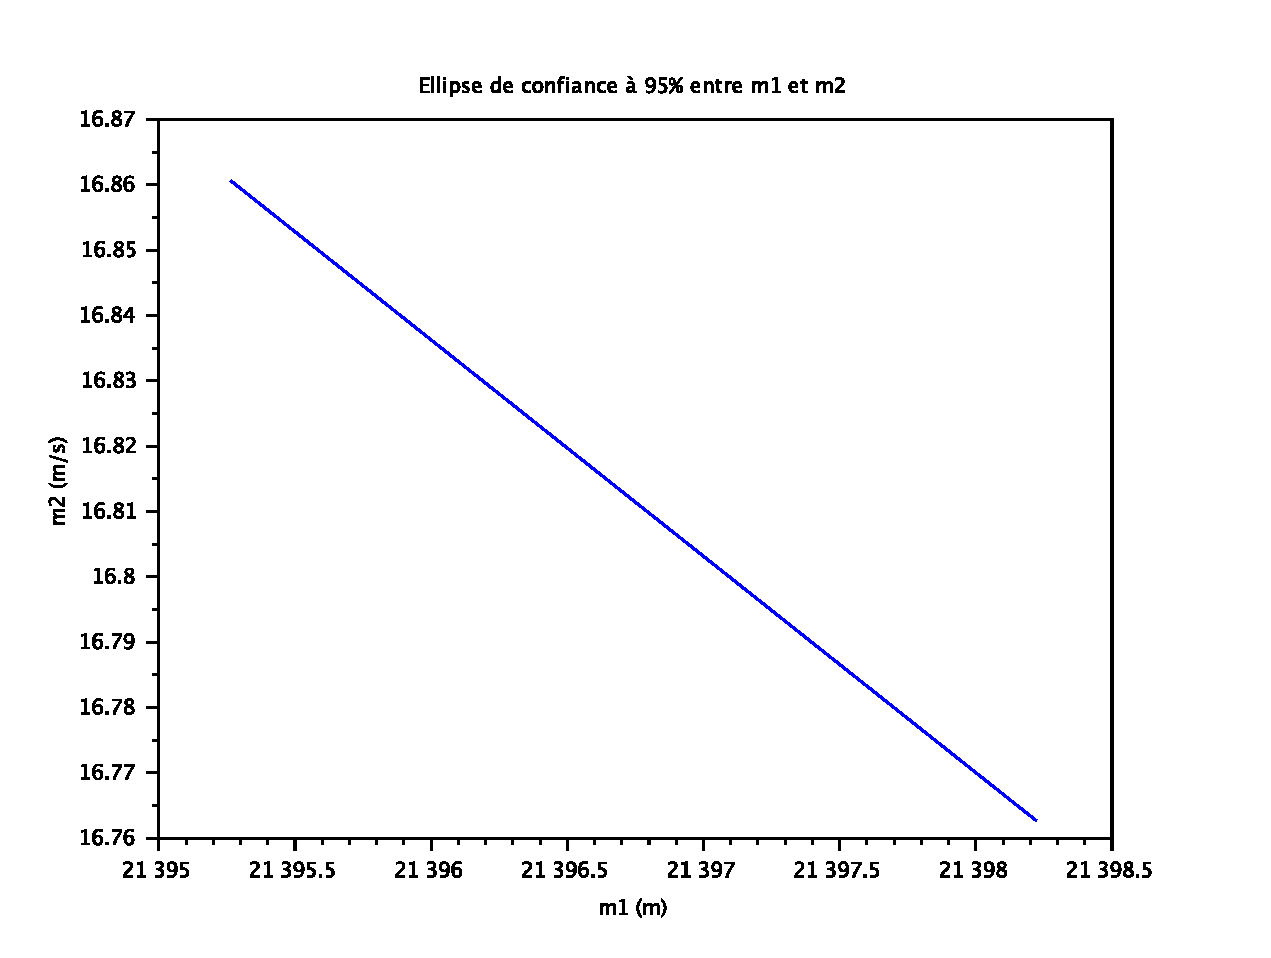
\includegraphics[width=12cm]{../m1m2.pdf} 
\end{center}
\caption{Ellipse de confiance à 0.95 entre m1 et m2}
\end{figure}
m1 et m2
\newpage

\begin{figure}[h]
\begin{center}
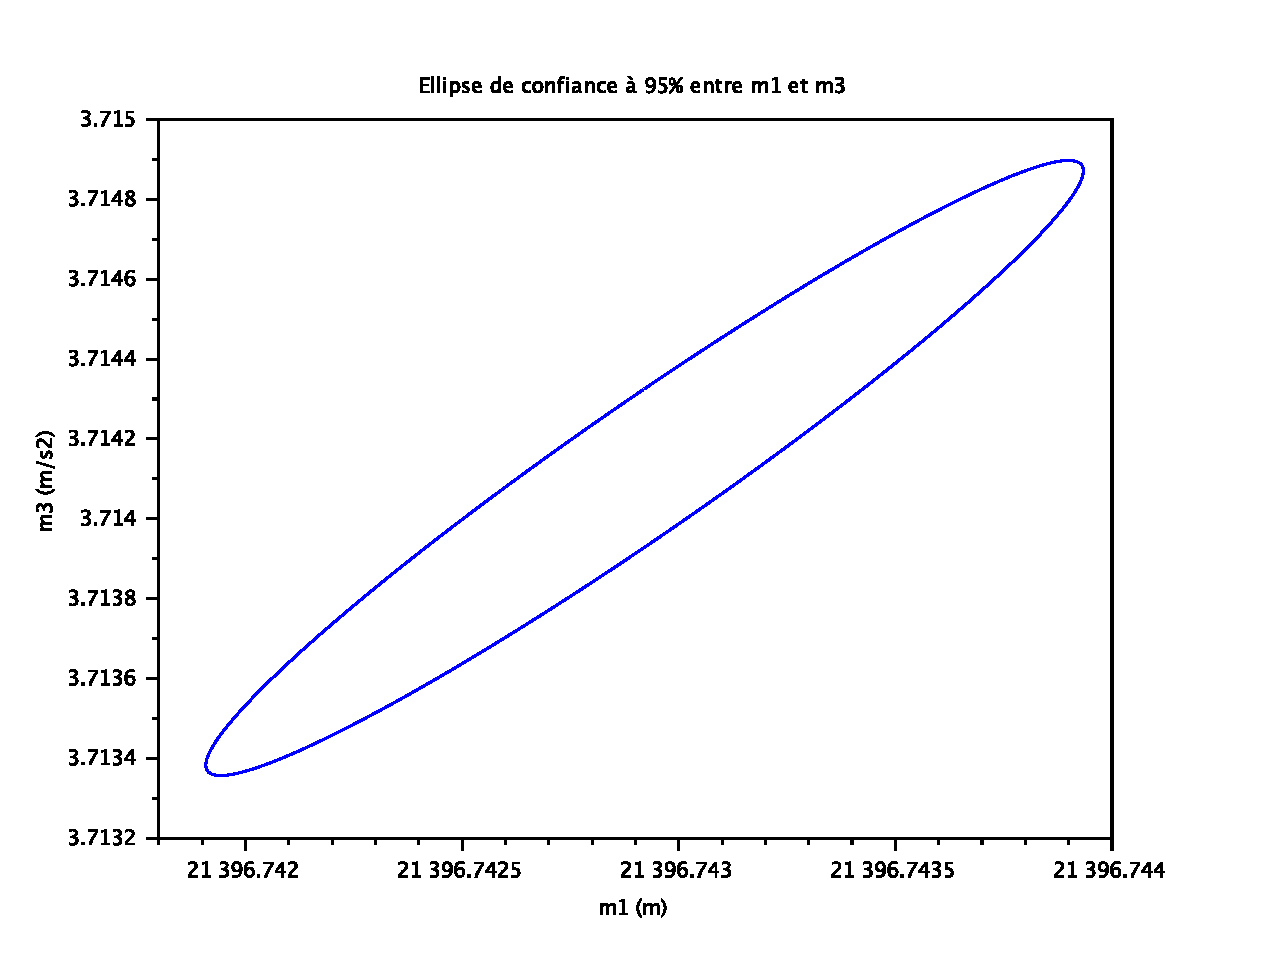
\includegraphics[width=12cm]{../m1m3.pdf} 
\end{center}
\caption{Ellipse de confiance à 0.95 entre m1 et m3}
\end{figure}
m1 et m3
\newpage

\begin{figure}[h]
\begin{center}
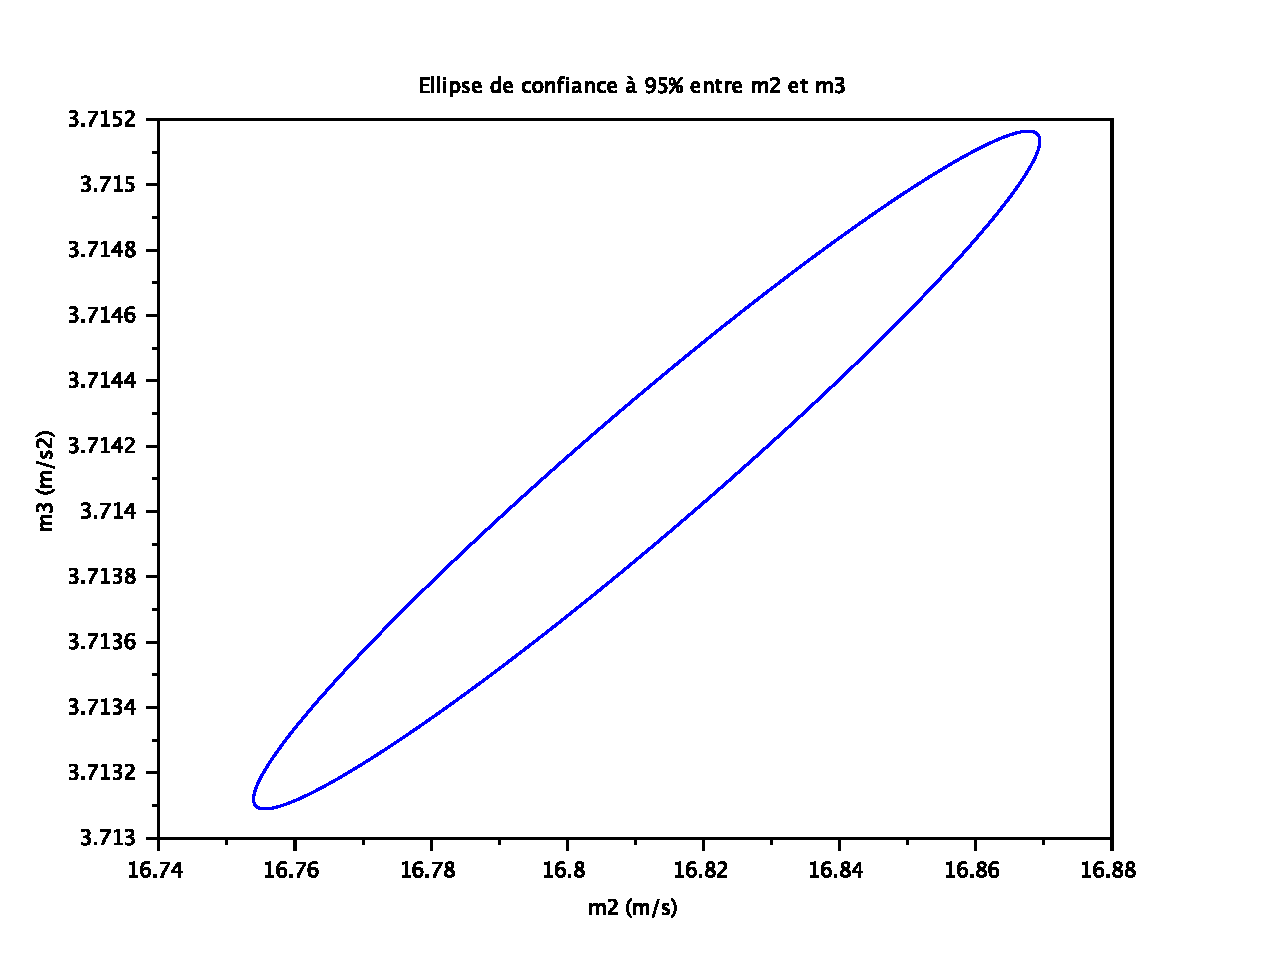
\includegraphics[width=12cm]{../m2m3.pdf} 
\end{center}
\caption{Ellipse de confiance à 0.95 entre m2 et m3}
\end{figure}
m2 et m3

\newpage
\section{Comparaison valeurs de (e) et (c)}
Les valeurs de (e) sont plus grandes car elles représentent la dispersion à 0.95 des couples de paramètres pris 2 à 2, alors que les valeurs de (c) représente la dispersion des valeurs de chacun des paramètres. Ces valeurs sont différentes car elles ne mesurent pas la même population de "points".

\section{Misfit: formule}
\begin{equation}
\phi(m) = \frac{1}{N}\sum_{i=1}^{N}(\frac{d_i^{observed}-d_i^{predicted}}{\sigma_i})^2
\end{equation}


\section{Misfit expected v}
La valeur du misfit est de 9339.5885 m.

\paragraph*{}
Cette valeur n'est pas zéro car elle représente la somme des carrés des différences entre les mesures et les valeurs prédites par le modèle calculé. 
\paragraph*{}
Les mesures étant bruitées, le misfit ne peut être zéro.

\section{Misfit: valeur attendue}

La valeur attendue du misfit dans cette formule est 1.

\section{Misfit avec $\sigma =0.5$ m}

Le misfit avec $\sigma=0.5$ m est de 37358.354 m.
\paragraph*{}
Nous en concluons que de passer le $\sigma$ de 1 à 0,5m augmente le misfit. L'ajustement du $\sigma$ ne doit pas se faire dans cette direction.

\section{Misfit avec $\sigma = 800 m $}

La valeur du msifit avec $\sigma = 800$m est de 0.0145931 m.

\paragraph{}
Cette valeur est beaucoup trop petite. $\sigma$ ne doit pas être aussi grand.
\section{Evaluation de la valeur de $\sigma$}

Nous pouvons essayer d'ajuster la valeur de $\sigma$ en calculant le misfit pour différentes valeurs de $\sigma$ pour tenter d'obtenir une valeur de $\phi(m)$ proche de 1:

\begin{equation}
	\begin{array}{c}
	
	\sigma \; \; \;\;\;\; \phi(m) \\
		 2.\; \;\;  2334.8971 \\

   4.\; \;\;   583.72428 \\

   10. \; \;\; 93.395885 \\

   20. \; \;\;  23.348971 \\

   50. \; \;\;  3.7358354 \\

   100. \; \;\; 0.9339588 \\

   200.  \; \;\; 0.2334897 \\

   400. \; \;\;  0.0583724 \\

   800. \; \;\;  0.0145931 \\
	\end{array}
\end{equation}
Avec les calculs ci-dessus, nous voyons que $\sigma \simeq 100$, $\phi(m) \simeq 1$.
Donc $\sigma \simeq 100$ est une bonne estimation de l'écart-type.

\section{Où l'expérience a-t-elle eu lieu?}
$m_3$ correspondant à l'accélération de pesanteur à la surface de la planète, nous constatons que sa valeur calculée ($3.714 m.s^{-2}$) est différente de celle de la Terre ($9,806 m.s{-2}$).

\paragraph*{}
Une recherche Wikipédia sur Mars nous indique que l'accélération de pesanteur à la surface de cette planète est de $3.711 m.s^{-2}$, très proche de notre valeur calculée.

\paragraph*{}
Par ailleurs, l'altitude de départ de l'expérience est de 21414m, ce qui équivaut à l'altitude du volcan le plus du haut du système solaire: Olympus Mons.

\paragraph*{}
L'expérience s'est donc déroulée sur la planète Mars, au sommet d'Olympus Mons.
\end{document}